\lstinputlisting[language=bash,basicstyle=\small]{python_codes/fieldstone_64/keywords.ascii}

\begin{center}
Code at \url{https://github.com/cedrict/fieldstone/tree/master/python_codes/fieldstone_64}
\end{center}

\par\noindent\rule{\textwidth}{0.4pt}
%%%%%%%%%%%%%%%%%%%%%%%%%%%%%%%%%%%%%%%%%%%%%%%%%%%%%%%%%%%%%%%%%%%%%%%%%%%%%%%%%%%%%%%%%%%%


{\large
DO NOT READ WHAT FOLLOWS. It was written for Composition based stone, but I am using 
markers for all benchmarks so far. Jump directly to 'stress build up in maxwell body'! 
}

In the examples here there are only 2 compositions. 
Each material/composition is characterised by its $\eta_{\{1,2\}}$, $\mu_{\{1,2\}}$. 
With $\delta t$ chosen, $Z_{\{1,2\}}$ and $\eta_{eff,\{1,2\}}$ can be computed.

C1 and C2 are initialised at startup by looping over Vnodes and assigning a value to $C_1$ 
and $C_2$ such that $C_1+C_2=1$. 

The quantity $\tau_{xx},\tau_{yy},\tau_{xy},\dot{\omega}_{xy}$ (denoted by oxy in the code) 
are nodal and initialised at startup
(they are needed for the Stokes matrix):
\begin{lstlisting}
tauxx =np.zeros(NV,dtype=np.float64)  
tauyy =np.zeros(NV,dtype=np.float64)  
tauxy =np.zeros(NV,dtype=np.float64)  
oxy   =np.zeros(NV,dtype=np.float64)  
etaeff=np.zeros(NV,dtype=np.float64)  
Z     =np.zeros(NV,dtype=np.float64)  
rho   =np.zeros(NV,dtype=np.float64)  
\end{lstlisting}

Structure of the code (the following bulletpoints are inside the time stepping loop):

\begin{itemize}
\item Nodal $\eta_{eff}$, $Z$ and $\rho$ values are computed as follows:
\begin{lstlisting}
for i in range(0,NV):
    etaeff[i]=C1[i]*etaeff1+C2[i]*etaeff2
    Z[i]     =C1[i]*Z1     +C2[i]*Z2
    rho[i]   =C1[i]*rho1   +C2[i]*rho2
\end{lstlisting}

\item Build Stokes matrix. 
Loop over elements, loop over integration points inside the element, and for 
each quadrature point:
\begin{eqnarray}
Z(\vec{r}_q) &=& \sum_{i=1}^{m_V} N_i^\upnu(\vec{r}_q) Z_i \\
\tau_{xx}(\vec{r}_q)&=& \sum_{i=1}^{m_V} N_i^\upnu(\vec{r}_q) \tau_{xx,i} \\
\tau_{yy}(\vec{r}_q)&=& \sum_{i=1}^{m_V} N_i^\upnu(\vec{r}_q) \tau_{yy,i} \\
\tau_{xy}(\vec{r}_q)&=& \sum_{i=1}^{m_V} N_i^\upnu(\vec{r}_q) \tau_{xy,i} \\
\eta_{eff}(\vec{r}_q)&=& \sum_{i=1}^{m_V} N_i^\upnu(\vec{r}_q) \eta_{eff,i} \\
\dot{\omega}_{xy}(\vec{r}_q) &=& \sum_{i=1}^{m_V} N_i^\upnu(\vec{r}_q)  \dot{\omega}_{xy,i} \\
\rho(\vec{r}_q) &=& \sum_{i=1}^{m_V} N_i^\upnu(\vec{r}_q) \rho_i 
\end{eqnarray}


The elastic memory rhs term is built following Eq.~(\ref{XXX}):
\begin{lstlisting}
R[0]=Zq*(tauxxq+dt*oxyq*(2*tauxyq))
R[1]=Zq*(tauyyq+dt*oxyq*(-2*tauxyq))
R[2]=Zq*(tauxyq+dt*oxyq*(tauyyq-tauxxq))
f_el-=b_mat.T.dot(R)*weightq*jcob
\end{lstlisting}

\item Solve system and obtain $u,v,p$

\item Compute nodal velocity gradient ${\bm L}=\vec\nabla\vec\upnu$

\item Compute derivated nodal fields 

\begin{lstlisting}
exx[:]=Lxx[:]
eyy[:]=Lyy[:]
exy[:]=0.5*(Lxy[:]+Lyx[:])
oxy[:]=0.5*(Lxy[:]-Lyx[:])
Jxx[:]=2*tauxx[:]*oxy[:]
Jyy[:]=-2*tauxy[:]*oxy[:]
Jxy[:]=(tauyy[:]-tauxx[:])*oxy[:]
\end{lstlisting}

\item (re-)build nodal ${\bm \tau}$: 
\begin{lstlisting}
tauxx=2*etaeff*exx+Z*tauxx+Z*dt*Jxx
tauyy=2*etaeff*eyy+Z*tauyy+Z*dt*Jyy
tauxy=2*etaeff*exy+Z*tauxy+Z*dt*Jxy
\end{lstlisting}

\item advect $C_1$, $C_2$, $\tau_{xx}$, $\tau_{yy}$ and $\tau_{xy}$ fields

\item produce vtu file

\end{itemize}





%.......................................................
\paragraph{About this code}

This is a fairly complicated code since it features a deformable mesh 
(by means of a simplified ALE which only allows for the vertical movement 
of only the top row of mesh nodes), a particle-in-cell technique (only 
1st order in space)
to carry out material tracking/advection and of course the elasto-viscous 
rheology.


%.......................................................
\paragraph{Stress build-up in viscoelastic Maxwell body - analytical solution}

We start from 
\[
\dot{\bm \varepsilon}_T = \dot{\bm \varepsilon}_e +\dot{\bm \varepsilon}_v
=\frac{1}{2\mu} \dot{\bm \tau} + \frac{1}{2\eta} {\bm \tau} 
\]
In the case where there is no rotation then the BLABLA derivative becomes $d/dt$
and then 
we have to solve 
\[
2 \mu \dot{\bm \varepsilon}_T 
= \frac{d {\bm \tau}}{dt} + \frac{\mu}{\eta} {\bm \tau}
= \frac{d {\bm \tau}}{dt} + \frac{{\bm \tau}}{t_M}
\]
where $t_M=\eta/mu$ is the Maxwell time. The general solution can be arrived at 
by means of the Laplace transform (?!) and is given by:
\[
{\bm \tau}(t) = {\bm \tau}(t_0) \exp\left( -\frac{t-t_0}{t_M} \right) + \exp \left(-\frac{t}{t_M}\right)
\int_{t_0}^{t} 2 \mu \dot{\bm \varepsilon}_T  \exp \left(\frac{t'}{t_M}\right) dt'
\]

If $t_0=$ and ${\bm \tau}(t_0)=0$ then
\[
{\bm \tau}(t) =  \exp \left(-\frac{t}{t_M}\right)
\int_{0}^{t} 2 \mu \dot{\bm \varepsilon}_T  \exp \left( \frac{t'}{t_M} \right) dt'
\]
If the strain rate and shear modulus are constant in time, then 
\begin{eqnarray}
{\bm \tau}(t) 
&=&  \exp \left(-\frac{t}{t_M}\right)
2 \mu \dot{\bm \varepsilon}_T   \int_{0}^{t} \exp \left( \frac{t'}{t_M} \right) dt' \nn\\
&=&  \exp \left(-\frac{t}{t_M}\right)
2 \mu \dot{\bm \varepsilon}_T  t_M  \left[ \exp \left( \frac{t}{t_M} \right) -1  \right] \nn\\
&=& 
2 \eta \dot{\bm \varepsilon}_T   \left[ 1 - \exp \left( -\frac{t}{t_M} \right)\right] \nn
\end{eqnarray}
since $t_M=\eta/\mu$.

%.......................................................
\paragraph{Stress build-up in viscoelastic Maxwell body under simple shear}

The first benchmark performed to test the viscoelastic implementation considers the stress 
build-up present in a viscoelastic Maxwell body. Contrary to stressed viscous materials, 
viscoelastic materials gradually build-up stress when sheared after which a transition to viscous deformation occurs.  

An unstressed, incompressible viscoelastic Maxwell medium is subjected to a velocity field 
resulting in pure shear. 
The increase of the accumulated stress with time is given by an analytical solution:
\begin{equation}
{\bm \tau} = 2\eta\ {\dot{\bm \varepsilon}} \left ( 1-e^{-\frac{\mu }{\eta} t } \right )
\end{equation}
with $t$ time, $\eta$ the prescribed material viscosity and $\mu$ the prescribed material shear modulus. 
The domain size is 100$\times 100$km.
The velocity prescribed at all boundaries equals $v=1$ cm/yr in magnitude yielding a constant 
background strain rate of $\dot{\varepsilon}=2\text{cm/yr}/100\text{km}\simeq 6.342\times 10^{-15}$. 
The viscosity is $\eta= 10^{21}\text{Pa.s}$, the shear modulus is 
$\mu =10^{10}$Pa and the gravity is set to zero. We set $\delta t=100$yr.  

\begin{center}
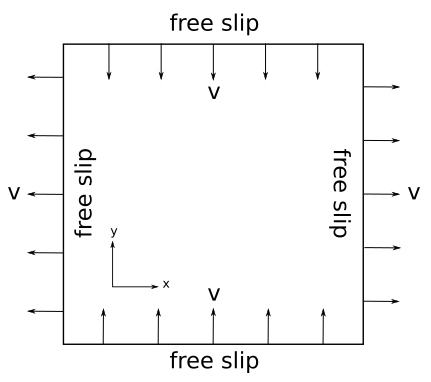
\includegraphics[width=5cm]{python_codes/fieldstone_64/images/stress_buildup_setup.png}\\
\captionfont{
Set up of the stress build-up benchmark. All domain sides have a free slip
boundary condition, and pure shear velocity conditions are prescribed. Adapted from 
Gerya (2010) \cite{gery10}.} 
\end{center}

We have 
\[
\eta_{eff} 
= \frac{\eta \delta t}{\delta t + \eta/\mu} 
= \frac{10^{21} \cdot 3.154\times 10^{9}}{3.154\times 10^{9} + 10^{21}/10^{10}} 
\simeq 
3.0592 \times 10^{19}\text{Pa.s}
\qquad
\text{and}
\qquad
Z=\frac{\eta_{eff}}{\mu \delta t} 
\simeq 
0.9694
\]
The Maxwell time is $t_M = \frac{\eta}{\mu} = 10^{11}\text{s} \simeq 3171\text{yr}$.
In the absence of elasticity (purely viscous behaviour), we have 
$\dot{\varepsilon}_{xx} = 6.342\times 10^{-15}$ 
and $\eta=10^{21}$ so the 
deviatoric stress $\tau_{xx}$ is equal to 
\[
\tau_{xx} = 2 \cdot 10^{21} \cdot 6.342\times 10^{-15} \simeq 12.68 \times 10^6 \text{Pa}
\]

The first time that the Stokes system is solved, there is no stored stress, i.e. the 
elastic rhs is identically zero, so that the system is solved with a viscosity equal to
$\eta_{eff}$.
We can easily compute the analytical solution, and we see that $\dot{\varepsilon}_{xy}=0$
and $\dot{\omega}_{xy}=0$, which we recover:

\begin{center}
\includegraphics[width=5cm]{python_codes/fieldstone_64/results/buildup_11/init/vel}
\includegraphics[width=5cm]{python_codes/fieldstone_64/results/buildup_11/init/exy}
\includegraphics[width=5cm]{python_codes/fieldstone_64/results/buildup_11/init/oxy}
\end{center}

The expected stress value for $\tau_{xx}$ after the first Stokes solve is 
\[
\tau_{xx} = 2 \eta_{eff} \dot{\varepsilon}_{xx} 
= 2 \cdot 3.057\times 10^{19} \cdot 6.342\times 10^{-15} 
\simeq 38.775 \times 10^4 \text{Pa}
\]

\begin{center}
\includegraphics[width=9cm]{python_codes/fieldstone_64/results/buildup_11/tauxx}\\
{\captionfont $\tau_{xx}$ as a function of time.}
\end{center}

\includegraphics[width=5cm]{python_codes/fieldstone_64/results/buildup_11/tau}
\includegraphics[width=5cm]{python_codes/fieldstone_64/results/buildup_11/strainrate}
\includegraphics[width=5cm]{python_codes/fieldstone_64/results/buildup_11/velocity}\\

\begin{remark}
Because of the outflux boundary conditions it can happen that some markers 
exit the domain. In order to avoid dealing with these, markers are artificially 
kept inside the domain (near the boundary).
\end{remark}

%.......................................................
\paragraph{Stress build-up in viscoelastic Maxwell body under simple shear}

I have also created a similar problem, although this time simple shear boundary conditions are prescribed.
$v=0$ on left and right boundary, (-1,0)cm/yr at the bottom, (+1,0)cm/yr at the top.

ANALYTICAL SOLUTION!?!
$\tau_{xy} \rightarrow 2 \eta \dot{\varepsilon}_xy = 6.342\times 10^{6} Pa$ 

\begin{center}
\includegraphics[width=5cm]{python_codes/fieldstone_64/results/buildup_12/vel}
\end{center}

In simple shear, we have $\dot{\varepsilon}_{xx}=\dot{\varepsilon}_{yy}=0$, and 
\[
\dot{\varepsilon}_{xy}=\frac{1}{2} \frac{\Delta u}{L_y} = \frac{1 cm/yr}{100km}
\]

\begin{center}
\includegraphics[width=9cm]{python_codes/fieldstone_64/results/buildup_12/tauxy}\\
{\captionfont $\tau_{xy}$ as a function of time.}
\end{center}

\includegraphics[width=5cm]{python_codes/fieldstone_64/results/buildup_12/tau}
\includegraphics[width=5cm]{python_codes/fieldstone_64/results/buildup_12/strainrate}
\includegraphics[width=5cm]{python_codes/fieldstone_64/results/buildup_12/velocity}\\




%........................
\paragraph{Bending of elastic slab}

The sinking slab benchmark consists of a beam of elastic material which is placed 
in a weak and viscous surrounding medium. The initially unstressed beam is attached 
to the left domain boundary through boundary conditions. A stress is then applied to 
the beam in the form of gravity. The applied gravity force results in the deformation 
of the beam through bending. After 20 kyr, the gravity field is turned off and the 
elastic properties of the beam will then force itself to its original position.  
The set-up of the benchmark is given in the following figure: 

\begin{center}
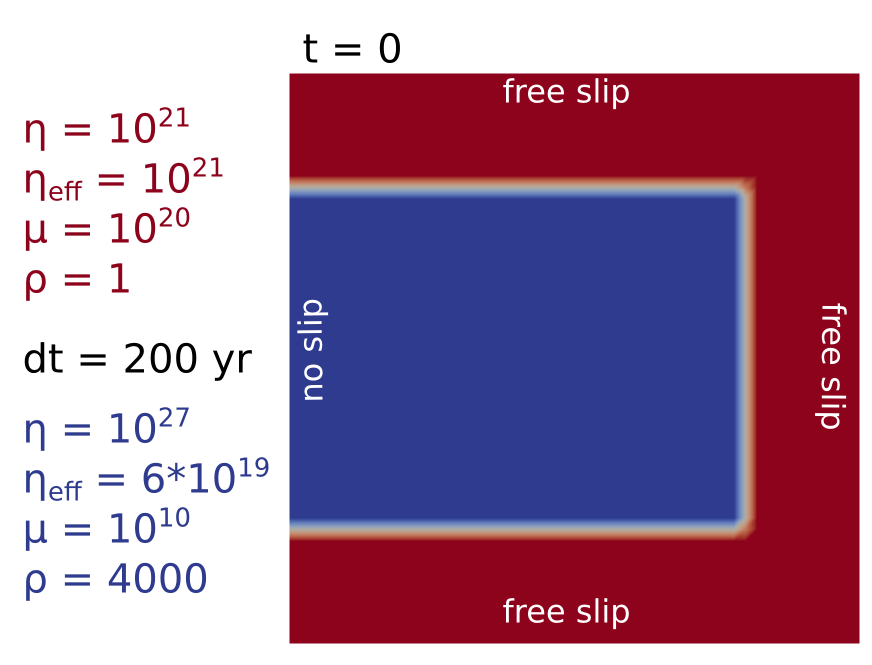
\includegraphics[width=6cm]{python_codes/fieldstone_64/images/poster_benchmark.png}\\
\captionfont{Set-up of the benchmark from \cite{gery10}. The properties of the 
two materials are given on the left, together\\ with the initial configuration of the benchmark.} 
\end{center}

The beam is surrounded by a low-density, low-viscosity and high shear modulus medium 
of which the specifications are given in  the following table.
The boundary conditions of the domain consist of a no slip condition at 
the left boundary where the slab is attached and free slip boundary conditions along all other sides. 
The results are calculated on a grid with a resolution of 50x50 elements containing 64 randomly 
distributed markers at startup.
The time step is set to $\delta t = 200yr$ (i.e. gravity is switched off after 100 time steps).

\begin{center}
\begin{tabular}{lll}
\hline 
\textit{Material properties}& \textit{Elastic slab (fluid 1)}  & \textit{Surrounding medium (fluid 2)} \\
\hline 
\hline 
Density         $\rho$ \     [kg/m$^{3}$]      & 4000                    & 1     \\
Viscosity       $\eta$ \    [Pa$\cdot$ s]      & $10^{27}$               &   $10^{21}$     \\
Shear modulus   $\mu $ \    [Pa]               & $10^{10}$               & $10^{20}$       \\
Maxwell time $t_M$     \    [yr]               & 3.17Gyr                 &  $3.17\times10^{-7}$yr       \\
eff. visc.      $\eta_{eff}$ \ [Pa$\cdot$s]    & 6.307199602192306e+19   &  9.999999984145105e+20      \\
visco-elasticity factor $Z$      \ [-]         & 0.9999999369280039      &  1.5854895966744522e-09     \\
\hline 
\end{tabular} 
\end{center}

\begin{center}
\includegraphics[height=4.5cm]{python_codes/fieldstone_64/images/gerya1}
\includegraphics[height=4.5cm]{python_codes/fieldstone_64/images/gerya2}
\includegraphics[height=4.5cm]{python_codes/fieldstone_64/images/gerya3}\\
\includegraphics[height=4.5cm]{python_codes/fieldstone_64/results/slab/markers0000}
\includegraphics[height=4.5cm]{python_codes/fieldstone_64/results/slab/markers0100}\\
{\captionfont Top row taken from \cite[16.11]{gery10}. 
Results of a numerical experiment for the recovery of the original
shape of a visco-elastic slab (black, dark grey), 
 embedded in a weak visco-elastic medium (light grey, white). 
(a) Initial configuration, (b) configuration after 20 Kyr of deformation under 
constant vertical gravity field ($g_x=0$,$g_y =-10\text{m/s}^2$, 
(c) configuration achieved within 9980 Kyr of spontaneous deformation after 
switching off gravity (i.e. after $g_x=g_z=0$ condition is applied at
20 Kyr). Numerical results are calculated at a resolution 51$\times$51 nodes and
200$\times$200 markers. Note the irreversible viscous deformation of the weak surrounding medium,
which is visible in its perturbed checkerboard structure close to slab corners in (c).}
\end{center}

\newpage
The first time that the Stokes system is solved, there is no stored stress, i.e. the 
elastic rhs is identically zero, and the system is solved with a viscosity equal to
$\eta_{eff,1}$ and $\eta_{eff,2}$ for the slab and mantle respectively:

\begin{center}
\includegraphics[width=5.2cm]{python_codes/fieldstone_64/results/slab/init/vel}
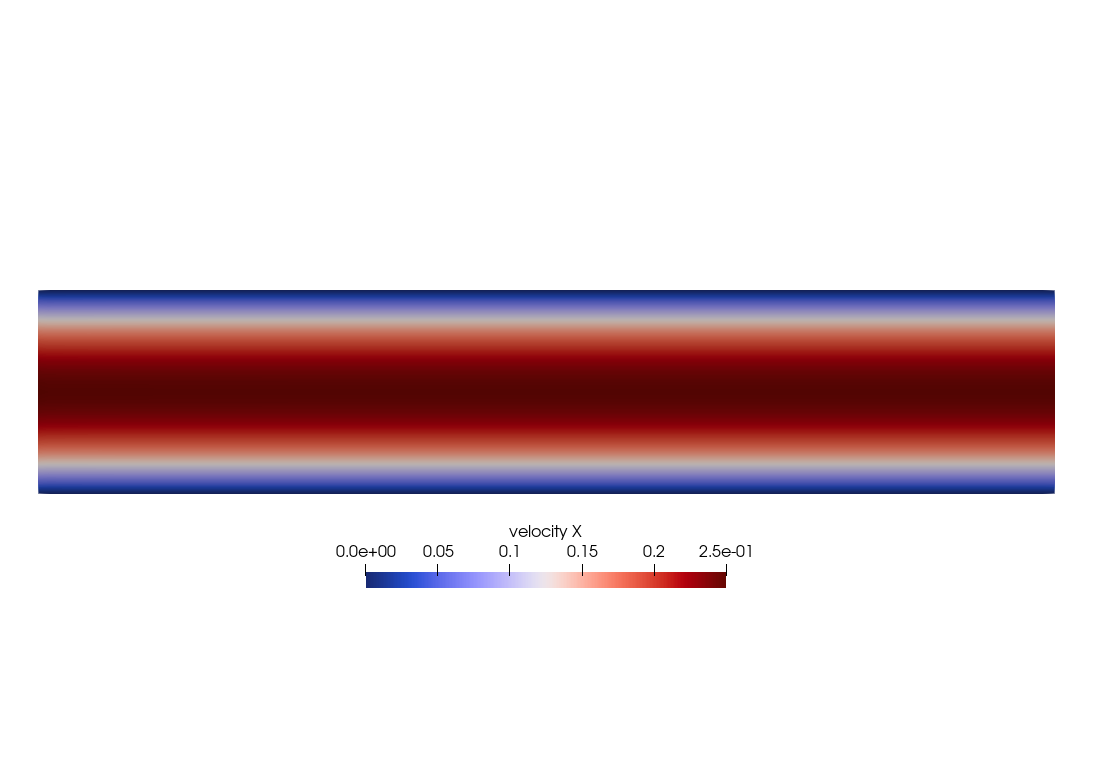
\includegraphics[width=5.2cm]{python_codes/fieldstone_64/results/slab/init/u}
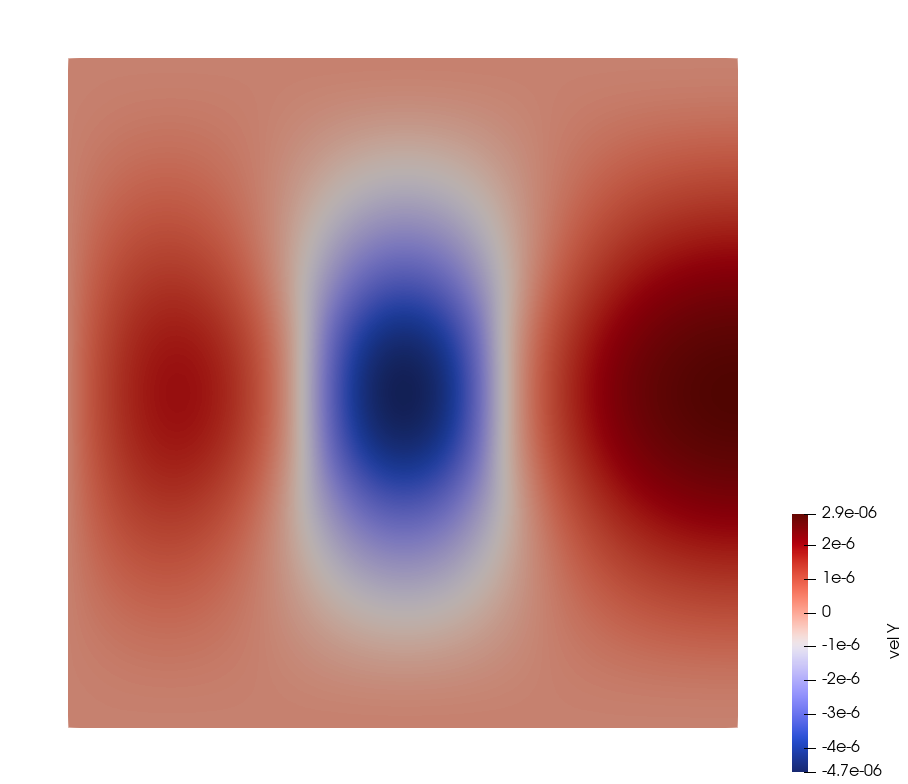
\includegraphics[width=5.2cm]{python_codes/fieldstone_64/results/slab/init/v}\\
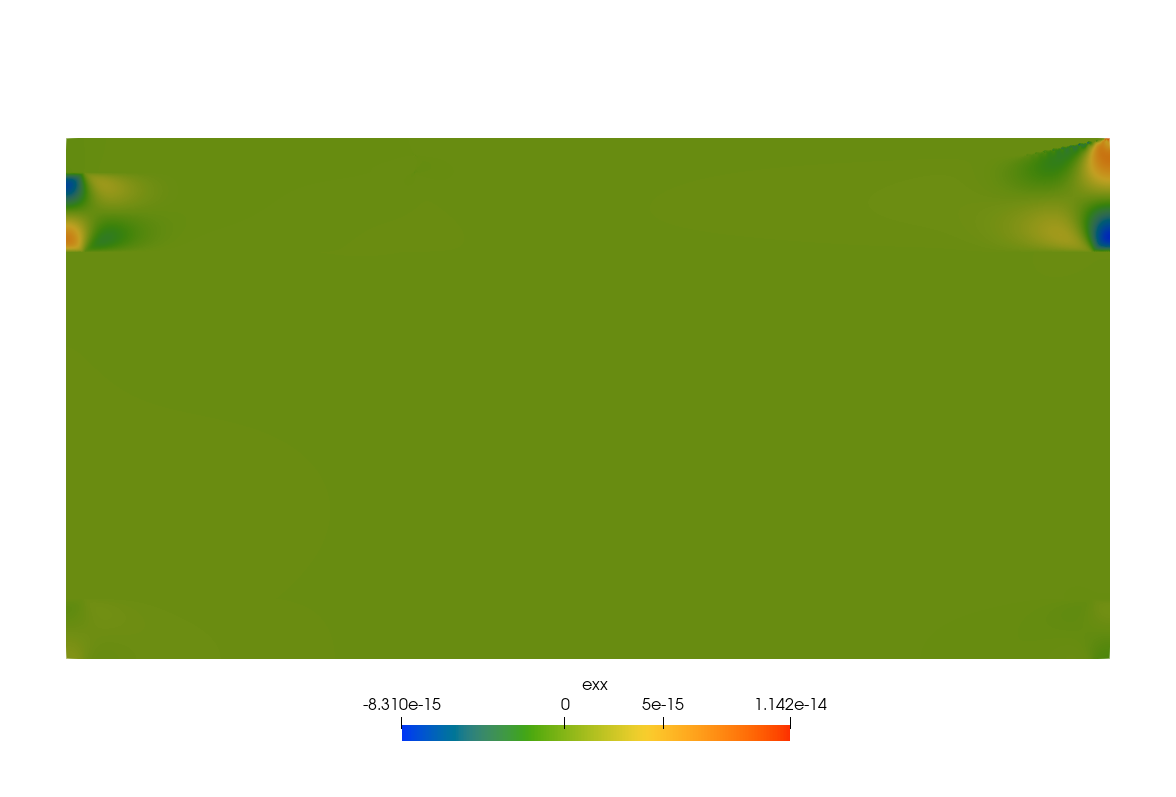
\includegraphics[width=5.2cm]{python_codes/fieldstone_64/results/slab/init/exx}
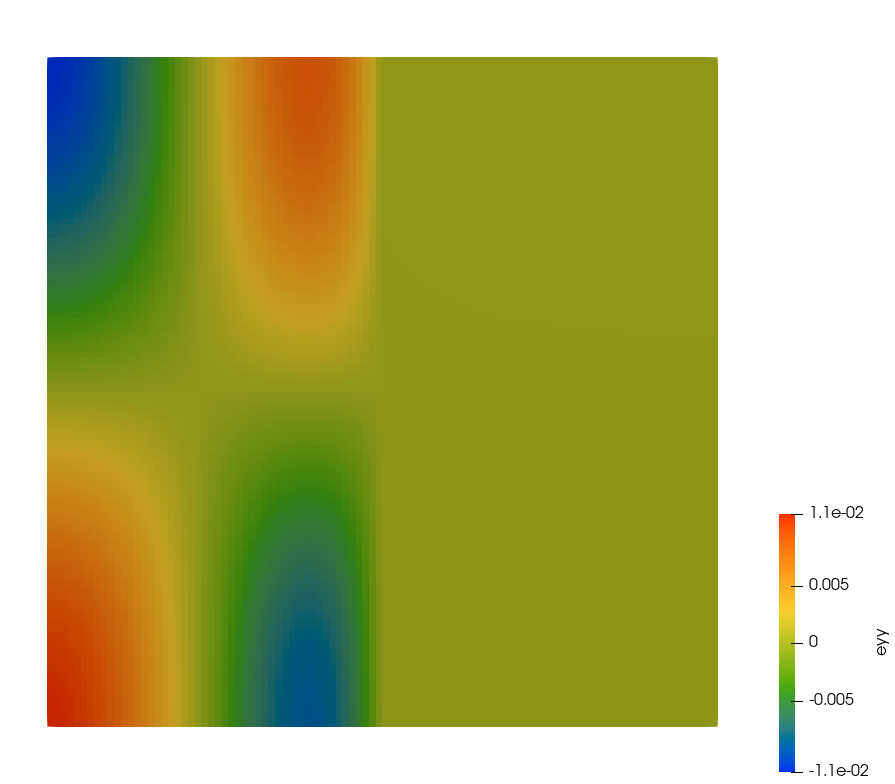
\includegraphics[width=5.2cm]{python_codes/fieldstone_64/results/slab/init/eyy}
\includegraphics[width=5.2cm]{python_codes/fieldstone_64/results/slab/init/exy}\\
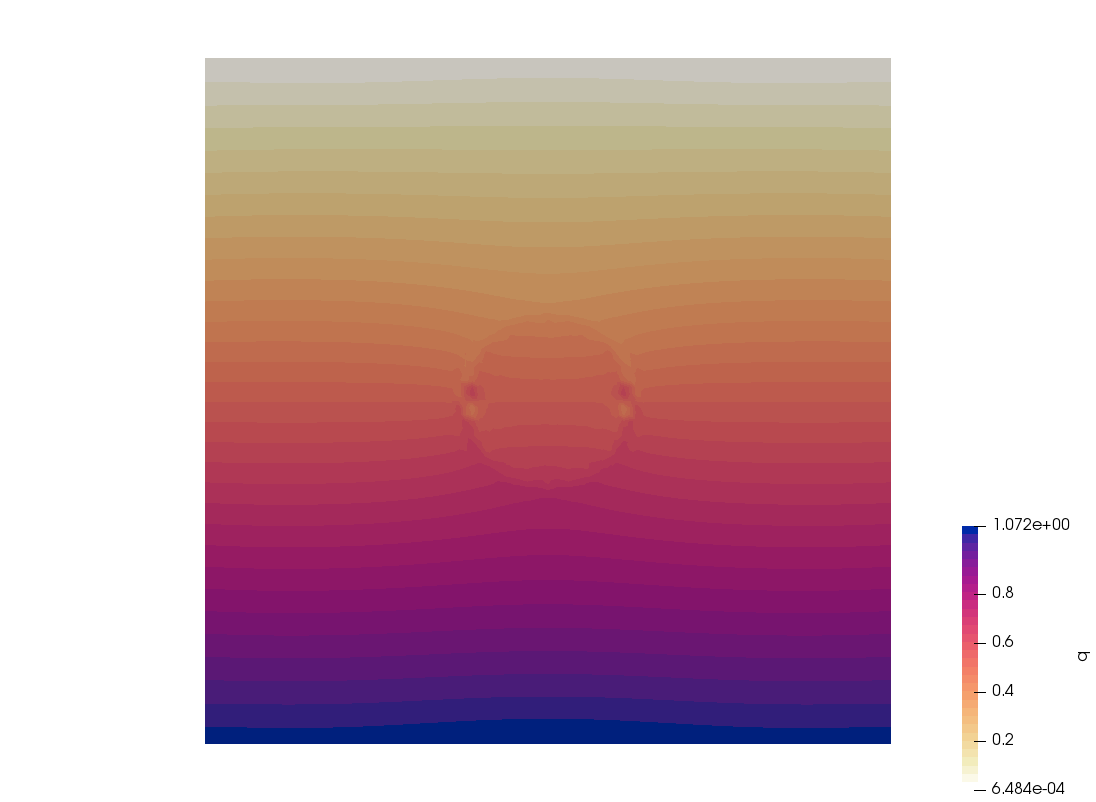
\includegraphics[width=5.2cm]{python_codes/fieldstone_64/results/slab/init/q}
\includegraphics[width=5.2cm]{python_codes/fieldstone_64/results/slab/init/etaeff}
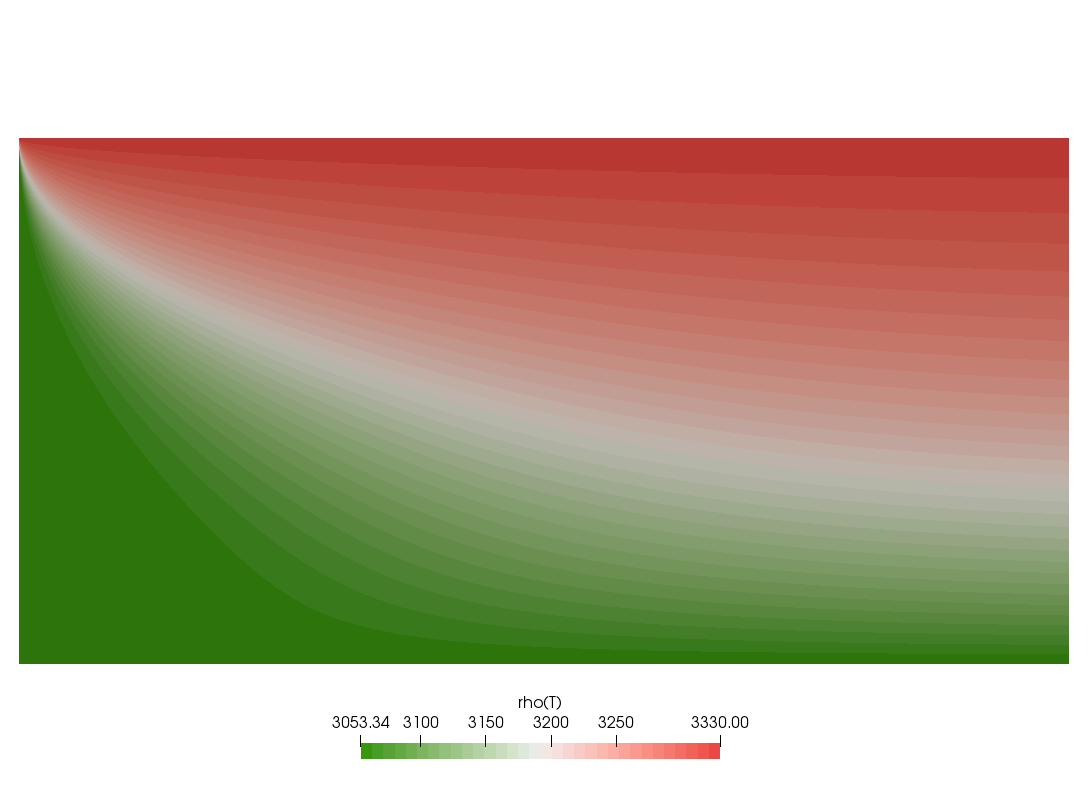
\includegraphics[width=5.2cm]{python_codes/fieldstone_64/results/slab/init/rho}
\end{center}

Note that the Gerya data are obtained with the code from the 2010 version of the book.

\begin{center}
\includegraphics[width=7cm]{python_codes/fieldstone_64/results/slab/velocity_u}
\includegraphics[width=7cm]{python_codes/fieldstone_64/results/slab/velocity_v}\\
\includegraphics[width=7cm]{python_codes/fieldstone_64/results/slab/J}
\includegraphics[width=7cm]{python_codes/fieldstone_64/results/slab/tau}
\end{center}


\newpage

\begin{center}
\includegraphics[width=5cm]{python_codes/fieldstone_64/results/slab/gerya2/markers_0000_Myr}
\includegraphics[width=5cm]{python_codes/fieldstone_64/results/slab/gerya2/stress_0000_Myr}
\includegraphics[width=5cm]{python_codes/fieldstone_64/results/slab/gerya2/velocity_0000_Myr}\\
\includegraphics[width=5cm]{python_codes/fieldstone_64/results/slab/gerya2/markers_0010_Myr}
\includegraphics[width=5cm]{python_codes/fieldstone_64/results/slab/gerya2/stress_0010_Myr}
\includegraphics[width=5cm]{python_codes/fieldstone_64/results/slab/gerya2/velocity_0010_Myr}\\
\includegraphics[width=5cm]{python_codes/fieldstone_64/results/slab/gerya2/markers_0020_Myr}
\includegraphics[width=5cm]{python_codes/fieldstone_64/results/slab/gerya2/stress_0020_Myr}
\includegraphics[width=5cm]{python_codes/fieldstone_64/results/slab/gerya2/velocity_0020_Myr}\\
\includegraphics[width=5cm]{python_codes/fieldstone_64/results/slab/gerya2/markers_0030_Myr}
\includegraphics[width=5cm]{python_codes/fieldstone_64/results/slab/gerya2/stress_0030_Myr}
\includegraphics[width=5cm]{python_codes/fieldstone_64/results/slab/gerya2/velocity_0030_Myr}\\
\includegraphics[width=5cm]{python_codes/fieldstone_64/results/slab/gerya2/markers_0040_Myr}
\includegraphics[width=5cm]{python_codes/fieldstone_64/results/slab/gerya2/stress_0040_Myr}
\includegraphics[width=5cm]{python_codes/fieldstone_64/results/slab/gerya2/velocity_0040_Myr}\\
\includegraphics[width=5cm]{python_codes/fieldstone_64/results/slab/gerya2/markers_0100_Myr}
\includegraphics[width=5cm]{python_codes/fieldstone_64/results/slab/gerya2/stress_0100_Myr}
\includegraphics[width=5cm]{python_codes/fieldstone_64/results/slab/gerya2/velocity_0100_Myr}\\
{\captionfont Results obtained with the Matlab code provided with Gerya (2019) \cite{gery19book}}
\end{center}

\newpage
%.......................................................
\paragraph{Stress build-up in viscoelastic Maxwell body}

This benchmark comes from Appendix B of Keller et al (2013) \cite{kemk13}.

The domain is $7.5\times5$km. A dominantly elastic beam is fixed to, and protrudes horizontally 
from the left wall of the model box. 
Surrounding the elastic beam is a viscous, but inelastic fluid. 
All boundaries are free slip, except for the left wall, which is set to no slip in 
order to keep the bending beam fixed to the wall. The beam has a higher density than the surrounding fluid and
thus will bend down elastically driven by gravity. After the beam has 
accumulated some elastic strain through bending down, gravity is switched off. 
If the stress evolution is implemented accurately, the elastic beam should now, 
free from the pull of gravity, move upwards again and restore its initial position. 

Material properties are as follows:
\begin{itemize}
\item beam: $\rho=1500$, $\eta=10^{24}$, $\mu=10^{10}$
\item fluid: $\rho=1000$, $\eta=10^{18}$, $\mu=10^{11}$
\end{itemize}

This choice of parameters leads to a Maxwell time 
$t_m = 0.32$ yr for the background fluid and Maxwell times of 
$t_m = 3.2$ Myr for the beam, meaning that the deformation in this benchmark problem, 
which occurs on a timescale of thousands to a million years, 
will lead to dominantly viscous deformation in the fluid, 
and dominantly elastic behaviour of the beam. 

Keller et al set the numerical resolution to $300\times200$ elements, 
with 16 markers per elements for stress advection. Such a resolution is 
not feasible with our simple python implementation so the resolution is
then set to $96\times64$. 

The following plot comes from \cite{kemk13}:
\begin{center}
\includegraphics[width=14cm]{python_codes/fieldstone_64/images/kemk13}
\end{center}

The elastic timestep is set to $\delta t_e=100$yr and the tectonic timestep is set to the same value.
This yields $\eta_{eff}=10^{18}$ in the fluid, and $\eta_{eff}\simeq 3.15\times 10^{19}$.
After 50kyr, the gravity ($|\vec{g}|=10$) is switched off and the model is ran for another 
500kyr.


\begin{center}
\includegraphics[width=5cm]{python_codes/fieldstone_64/results/beam/u.png}
\includegraphics[width=5cm]{python_codes/fieldstone_64/results/beam/v.png}
\includegraphics[width=5cm]{python_codes/fieldstone_64/results/beam/vel}\\
\includegraphics[width=5cm]{python_codes/fieldstone_64/results/beam/exx}
\includegraphics[width=5cm]{python_codes/fieldstone_64/results/beam/eyy}
\includegraphics[width=5cm]{python_codes/fieldstone_64/results/beam/exy}\\
\includegraphics[width=5cm]{python_codes/fieldstone_64/results/beam/q}
\includegraphics[width=5cm]{python_codes/fieldstone_64/results/beam/rho}
\includegraphics[width=5cm]{python_codes/fieldstone_64/results/beam/Z}\\
{\captionfont Various fields at the end of the 1st timestep: 
Velocity, strain rate components, $Z$, $\eta_{eff}$, strain rate components, pressure.}
\end{center}

\begin{center}
\includegraphics[width=7cm]{python_codes/fieldstone_64/results/beam/u.pdf}
\includegraphics[width=7cm]{python_codes/fieldstone_64/results/beam/u_log.pdf}\\
\includegraphics[width=7cm]{python_codes/fieldstone_64/results/beam/v.pdf}
\includegraphics[width=7cm]{python_codes/fieldstone_64/results/beam/v_log.pdf}
\end{center}

\begin{center}
\includegraphics[width=5cm]{python_codes/fieldstone_64/results/beam/tauxx.pdf}
\includegraphics[width=5cm]{python_codes/fieldstone_64/results/beam/tauyy.pdf}
\includegraphics[width=5cm]{python_codes/fieldstone_64/results/beam/tauxy.pdf}
\end{center}


\newpage
%.......................................................
\paragraph{Flexure of elastic plate}

This benchmark is presented in Choi et al (2013) \cite{chtl13}. 
The setup is as follows:

\begin{center}
\includegraphics[width=12cm]{python_codes/fieldstone_64/images/chtl13a}
\end{center}

\begin{center}
\begin{tabular}{llll}
\hline 
\textit{Material properties}& \textit{elastic plate (1)}  & \textit{elastic block (2)} & \textit{viscous mantle (3)} \\
\hline 
\hline 
Density         $\rho$       \ [kg/m$^{3}$]       & 2700&1890 &2700 \\ 
Viscosity       $\eta$       \ [Pa$\cdot$ s]      & $10^{35}$& $10^{35}$ & $10^{17}$ \\ 
Shear modulus   $\mu $       \ [Pa]               & $30\cdot10^9$& $30\cdot10^9$&  $10^{50}$ \\
Maxwell time    $t_M$        \ [yr]               & 10569930 &  10569930 & 3.1709791983764584e-41 \\ 
eff. visc.      $\eta_{eff}$ \ [Pa$\cdot$s]       & 4.73039776e+18& 4.73039776e+18&  1e+17\\ 
Factor          $Z$          \ [-]                & 0.9999995&  0.9999995 &  6.3419583e-42 \\ 
\hline 
\end{tabular} 
\end{center}

The value of $\eta_1=\eta_2=10^{35}$ for the elastic materials was obtained through personal communication. 
The value of $\mu_3=10^{50}$ for the viscous material ensures that $\eta_{eff}=\eta_3$.
Note that in the publication the authors test both compressible and incompressible 
formulations, but we restrict ourselves to incompressible results since our code cannot handle compressible behavior. 
I also use dt=5year.

The authors report a converged total relief of 306-308m:

\begin{center}
\includegraphics[width=8cm]{python_codes/fieldstone_64/images/chtl13b}
\end{center}

This benchmark requires either a sticky air layer (see Section~\ref{MMM-sss:stickyair})
on top of the plate or a deformable mesh (ALE formulation, see Section~\ref{MMM-sss:ale}).


\begin{center}
\includegraphics[width=5cm]{python_codes/fieldstone_64/results/flexureplate/u.png}
\includegraphics[width=5cm]{python_codes/fieldstone_64/results/flexureplate/v.png}
\includegraphics[width=5cm]{python_codes/fieldstone_64/results/flexureplate/vel.png}\\
{\captionfont Initial velocity field}
\end{center}

On the following figures I plot the topography and velocity statistics obtained with 
a resolution of $100\times35$ elements and 50 markers per element, next to 
results from Choi et al and/or results with my code \elefant \cite{thie14}.  
\begin{center}
\includegraphics[width=5cm]{python_codes/fieldstone_64/results/flexureplate/topo.pdf}
\includegraphics[width=5cm]{python_codes/fieldstone_64/results/flexureplate/v.pdf}
\includegraphics[width=5cm]{python_codes/fieldstone_64/results/flexureplate/v_log.pdf}
\end{center}

\begin{center}
\includegraphics[width=5cm]{python_codes/fieldstone_64/results/flexureplate/tauxx}
\includegraphics[width=5cm]{python_codes/fieldstone_64/results/flexureplate/tauyy}
\includegraphics[width=5cm]{python_codes/fieldstone_64/results/flexureplate/tauxy}\\
{\captionfont accumulated deviatoric stress at time t=500yr on the markers.}
\end{center}


\begin{center}
\includegraphics[width=16cm]{python_codes/fieldstone_64/results/flexureplate/grid}\\
{\captionfont Grid at time t=500yr}
\end{center}


%The following figure shows the grid at equilibrium and the markers:

%\begin{center}
%\includegraphics[width=8cm]{FLEXTURE_OF_ELASTIC_PLATE/mats.png}
%\includegraphics[width=8cm]{FLEXTURE_OF_ELASTIC_PLATE/DevStressInv.png}\\
%\includegraphics[width=8cm]{FLEXTURE_OF_ELASTIC_PLATE/maxwelltime.png}
%\includegraphics[width=8cm]{FLEXTURE_OF_ELASTIC_PLATE/mu_ve}\
%\end{center}


\newpage
%.......................................................
\paragraph{Ice load}

The domain is $500\times500$km. Vertical gravity is 9.8, density is 3300, viscosity 
is $3\cdot10^{20}$, shear modulus is $10^{10}$, free slip on left, right and bottom. 
A normal stress is imposed on the top for $0<x<100$km. It corresponds to 
an ice sheet of density $\rho_i=900$ of 1000m height. 
The timestep is set to 100yr. Resolution is set to $50\times50$ elements.
Stress/traction b.c. are explained in Section~\ref{MMM-ss:openbc}.

Analytical solution is provided in Nakiboglu and Lambeck (1982) \cite{nala82}. 
Note however that this is a 2D setup while the original solution is for a 
cylindrical load and also for a semi-infinite domain.

\[
\eta_{eff} = \frac{\eta \delta t}{\delta t + \eta/\mu}
= 2.85362675546547e+19
\]

\begin{center}
\includegraphics[width=10cm]{python_codes/fieldstone_64/results/icesheetload/vel}\\
{\captionfont Left: ASPECT; Right: stone 64}
\end{center}


\begin{center}
\includegraphics[width=6cm]{python_codes/fieldstone_64/results/icesheetload/topo3}
\includegraphics[width=6cm]{python_codes/fieldstone_64/results/icesheetload/vel_stats}
\end{center}

\includegraphics[width=5cm]{python_codes/fieldstone_64/results/icesheetload/tauxx}
\includegraphics[width=5cm]{python_codes/fieldstone_64/results/icesheetload/tauyy}
\includegraphics[width=5cm]{python_codes/fieldstone_64/results/icesheetload/tauxy}
